\documentclass[sigconf]{acmart}

\usepackage{booktabs} % For formal tables

%\usepackage{makeidx}  % allows for indexgeneration
\usepackage{graphicx}
	\graphicspath{{images/}} 
%\usepackage{cite}
\usepackage{courier}
\usepackage{hyperref}
    \hypersetup{colorlinks=true,allcolors=blue}
\usepackage{listings}
	\lstset{
  		basicstyle=\ttfamily,
  		frame=none,
  		breaklines=true,
  		numbers=left,
  		xleftmargin=2em,
  		framexleftmargin=0em,
    	emphstyle=\textbf,
    	float=t
	}
	\lstdefinestyle{cbp-xml}{
	    basicstyle=\ttfamily\scriptsize,
  		emph={
        	register, create, add, to, resource,
        	from, eattribute, remove, ereference,
        	set, unset, session, Roy, Jen,
        	Moss, Richmond
    	}
	}
	\lstdefinestyle{eol}{
	    basicstyle=\ttfamily\scriptsize,
  		emph={
        	var, new, for, in
    	}
	}

% Copyright
%\setcopyright{none}
%\setcopyright{acmcopyright}
%\setcopyright{acmlicensed}
\setcopyright{rightsretained}
%\setcopyright{usgov}
%\setcopyright{usgovmixed}
%\setcopyright{cagov}
%\setcopyright{cagovmixed}


% DOI
\acmDOI{10.475/123_4}

% ISBN
\acmISBN{123-4567-24-567/08/06}

%Conference
\acmConference[ICSE'18]{International Conference on Software Engineering}{May-June 2018}{Gothenburg, Sweden} 
\acmYear{2018}
\copyrightyear{2018}

\acmPrice{15.00}


\begin{document}
\renewcommand{\thelstlisting}{\arabic{lstlisting}}
\renewcommand{\labelitemi}{$\bullet$}
\newcommand{\ts}{\textsuperscript}

\title{Optimising Change-based Model's Loading Performance}
%\titlenote{Produces the permission block, and copyright information}
%\subtitle{Extended Abstract}
%\subtitlenote{The full version of the author's guide is available as
%  \texttt{acmart.pdf} document}


\author{Alfa Yohannis}
%\authornote{}
%\orcid{1234-5678-9012}
\affiliation{%
  \institution{Computer Science Department University of York}
  \streetaddress{Heslington}
  \city{York} 
  %\state{Ohio} 
  \postcode{YO10 5GH}
  \country{United Kingdom} 
}
\email{ary506@york.ac.uk}

\author{Dimitris Kolovos}
%\authornote{}
\affiliation{%
  \institution{Computer Science Department University of York}
  \streetaddress{Heslington}
  \city{York} 
  %\state{Ohio}
  \country{United Kingdom} 
  \postcode{YO10 5GH}
}
\email{dimitris.kolovos@york.ac.uk}

\author{Fiona Polack}
%\authornote{}
\affiliation{%
  \institution{Computer Science Department University of York}
  \streetaddress{Heslington}
  \city{York} 
  %\state{Ohio}
  \country{United Kingdom} 
  \postcode{YO10 5GH}
}
\email{fiona.polack@york.ac.uk}

% The default list of authors is too long for headers}
\renewcommand{\shortauthors}{A. Yohannis et al.}


\begin{abstract}
This paper provides a sample of a \LaTeX\ document which conforms,
somewhat loosely, to the formatting guidelines for
ACM SIG Proceedings.\footnote{This is an abstract footnote}
\end{abstract}

%
% The code below should be generated by the tool at
% http://dl.acm.org/ccs.cfm
% Please copy and paste the code instead of the example below. 
%

\begin{CCSXML}
<ccs2012>
<concept>
<concept_id>10011007.10010940.10010971.10010980.10010984</concept_id>
<concept_desc>Software and its engineering~Model-driven software engineering</concept_desc>
<concept_significance>500</concept_significance>
</concept>
<concept>
<concept_id>10011007.10010940.10011003.10011002</concept_id>
<concept_desc>Software and its engineering~Software performance</concept_desc>
<concept_significance>300</concept_significance>
</concept>
<concept>
<concept_id>10011007.10010940.10010971.10010972</concept_id>
<concept_desc>Software and its engineering~Software architectures</concept_desc>
<concept_significance>100</concept_significance>
</concept>
</ccs2012>
\end{CCSXML}

\ccsdesc[500]{Software and its engineering~Model-driven software engineering}
\ccsdesc[300]{Software and its engineering~Software performance}
\ccsdesc[100]{Software and its engineering~Software architectures}

\keywords{ACM proceedings, \LaTeX, text tagging}


\maketitle

\section{Introduction}

\section{Change-based Models}

\section{Events}

\section{Model History}

\section{Optimisation Principles}


\subsection{The Last Value is All that Matters}
Lst. \ref{lst:set_attribute_eol} shows an EOL code to create a model. It performs set and unset operations to an attribute \texttt{name} of an object \texttt{node}. When executed, this code produces a CBP XML representation consists of 6 events shown in Lst. \ref{lst:set_attribute_cbp}. The 1\ts{st} event registers the package \texttt{node} and is followed by other events that create an object, with id "0", as an instance of a \texttt{Node} class (line 1) and then add the object to the model's resource to make the object a part of the model (line 2). The code then sets the attribute \texttt{name}'s value to "Old Name!" (line 3), then nullify/unset it (line 4), and finally sets it to "New Name!" as its latest value (line 5). Lst. \ref{lst:set_attribute_eol} shows that the last value's of \texttt{node.name} is all that matters (line 4). Any previous value assignment to the \texttt{name} attribute can be ignored (line 1 and 2), since the final version of the model will always be the same. 

\begin{lstlisting}[style=eol,caption={The EOL code for Setting  Attribute.},label=lst:set_attribute_eol]
var node = new Node;
node.name = "Old Name!";
node.name = null;
node.name = "New Name!";
\end{lstlisting}

\begin{lstlisting}[style=cbp-xml,caption={The generated change-based representation of Lst. \ref{lst:set_attribute_eol}. },label=lst:set_attribute_cbp]
0 <register epackage="node"/>
1 <create eclass="Node" epackage="node" id="0"/>
2 <add-to-resource position="0"><value eobject="0"/></add-to-resource>
3 <set-eattribute name="name" target="0"><value literal="Old Name!"/></set-eattribute>
4 <unset-eattribute name="name" target="0"/>
5 <set-eattribute name="name" target="0"><value literal="New Name!"/></set-eattribute>
\end{lstlisting}

All events that involve the object "0" are recorded in an object history. The object history records the line number of occurrence of each event (Lst. \ref{lst:set_attribute_eobject_history}). For example, \texttt{SetEAttributeValue} event contains line 3 and 5 based on its occurrence. 

\begin{lstlisting}[style=cbp-xml,caption={The event-line relationships recorded by an EObjectHistory of Lst. \ref{lst:set_attribute_eol}. },label=lst:set_attribute_eobject_history]
EObject: 0
    CreateEObjectEvent = [[1]]
    AddToResourceEvent = [[2]]
    EAttribute:
        name:
            UnsetEAttributeEvent = [[4]]
            SetEAttributeEvent = [[3], [5]]
\end{lstlisting}

The history enables us to track which lines can be ignored for optimisation so that not every event is executed to produce the same model. From Lst. \ref{lst:set_attribute_eobject_history}, we can deduce that line 3 and 4 can be ignored since the \texttt{SetEAttributeValue}'s last event always sets the end value of the \texttt{name} attribute. 

\begin{lstlisting}[style=cbp-xml,caption={The optimised change-based Representation of Lst. \ref{lst:set_attribute_eol}. },label=lst:set_attribute_optimised_cbp]
0 <register epackage="node"/>
1 <create eclass="Node" epackage="node" id="0"/>
2 <add-to-resource position="0"><value eobject="0"/></add-to-resource>
5 <set-eattribute name="name" target="0"><value literal="New Name!"/></set-eattribute>
\end{lstlisting}

\subsection{Unset Ignores Itself and Its Previous Sets and Unsets}

\begin{lstlisting}[style=eol,caption={The EOL code for Nullyfying/Unsetting  Attribute.},label=lst:unset_attribute_eol]
var node = new Node;
node.name = "Old Name!";
node.name = null;
node.name = "New Name!";
node.name = null;
\end{lstlisting}

\begin{lstlisting}[style=cbp-xml,caption={The generated change-based representation of Lst. \ref{lst:unset_attribute_eol}. },label=lst:unset_attribute_cbp]
0 <register epackage="node"/>
1 <create eclass="Node" epackage="node" id="0"/>
2 <add-to-resource position="0"><value eobject="0"/></add-to-resource>
3 <set-eattribute name="name" target="0"><value literal="Old Name!"/></set-eattribute>
4 <unset-eattribute name="name" target="0"/>
5 <set-eattribute name="name" target="0"><value literal="New Name!"/></set-eattribute>
6 <unset-eattribute name="name" target="0"/>
\end{lstlisting}

\begin{lstlisting}[style=cbp-xml,caption={The event-line relationships recorded by an EObjectHistory of Lst. \ref{lst:unset_attribute_eol}. },label=lst:unset_attribute_eobject_history]
EObject: 0
    CreateEObjectEvent = [[1]]
    AddToResourceEvent = [[2]]
    EAttribute:
        name:
            UnsetEAttributeEvent = [[4], [6]]
            SetEAttributeEvent = [[3], [5]]
\end{lstlisting}

\begin{lstlisting}[style=cbp-xml,caption={The optimised change-based Representation of Lst. \ref{lst:unset_attribute_eol}. },label=lst:unset_attribute_optimised_cbp]
0 <register epackage="node"/>
1 <create eclass="Node" epackage="node" id="0"/>
2 <add-to-resource position="0"><value eobject="0"/></add-to-resource>
\end{lstlisting}

\section{Performance}

\begin{lstlisting}[style=eol,caption={The EOL code for creating deep tree of nodes.},label=lst:deep_tree_eol]
var eRoot = new Node;
eRoot.name = "0";
for(i in Sequence{1..40}){
    var node = new Node;
    node.name = i.asString();
    eRoot.valNodes.add(node);
	   eRoot = node;
}
\end{lstlisting}

\subsection{Loading Deep Tree}
\begin{figure}[b!]
\centering
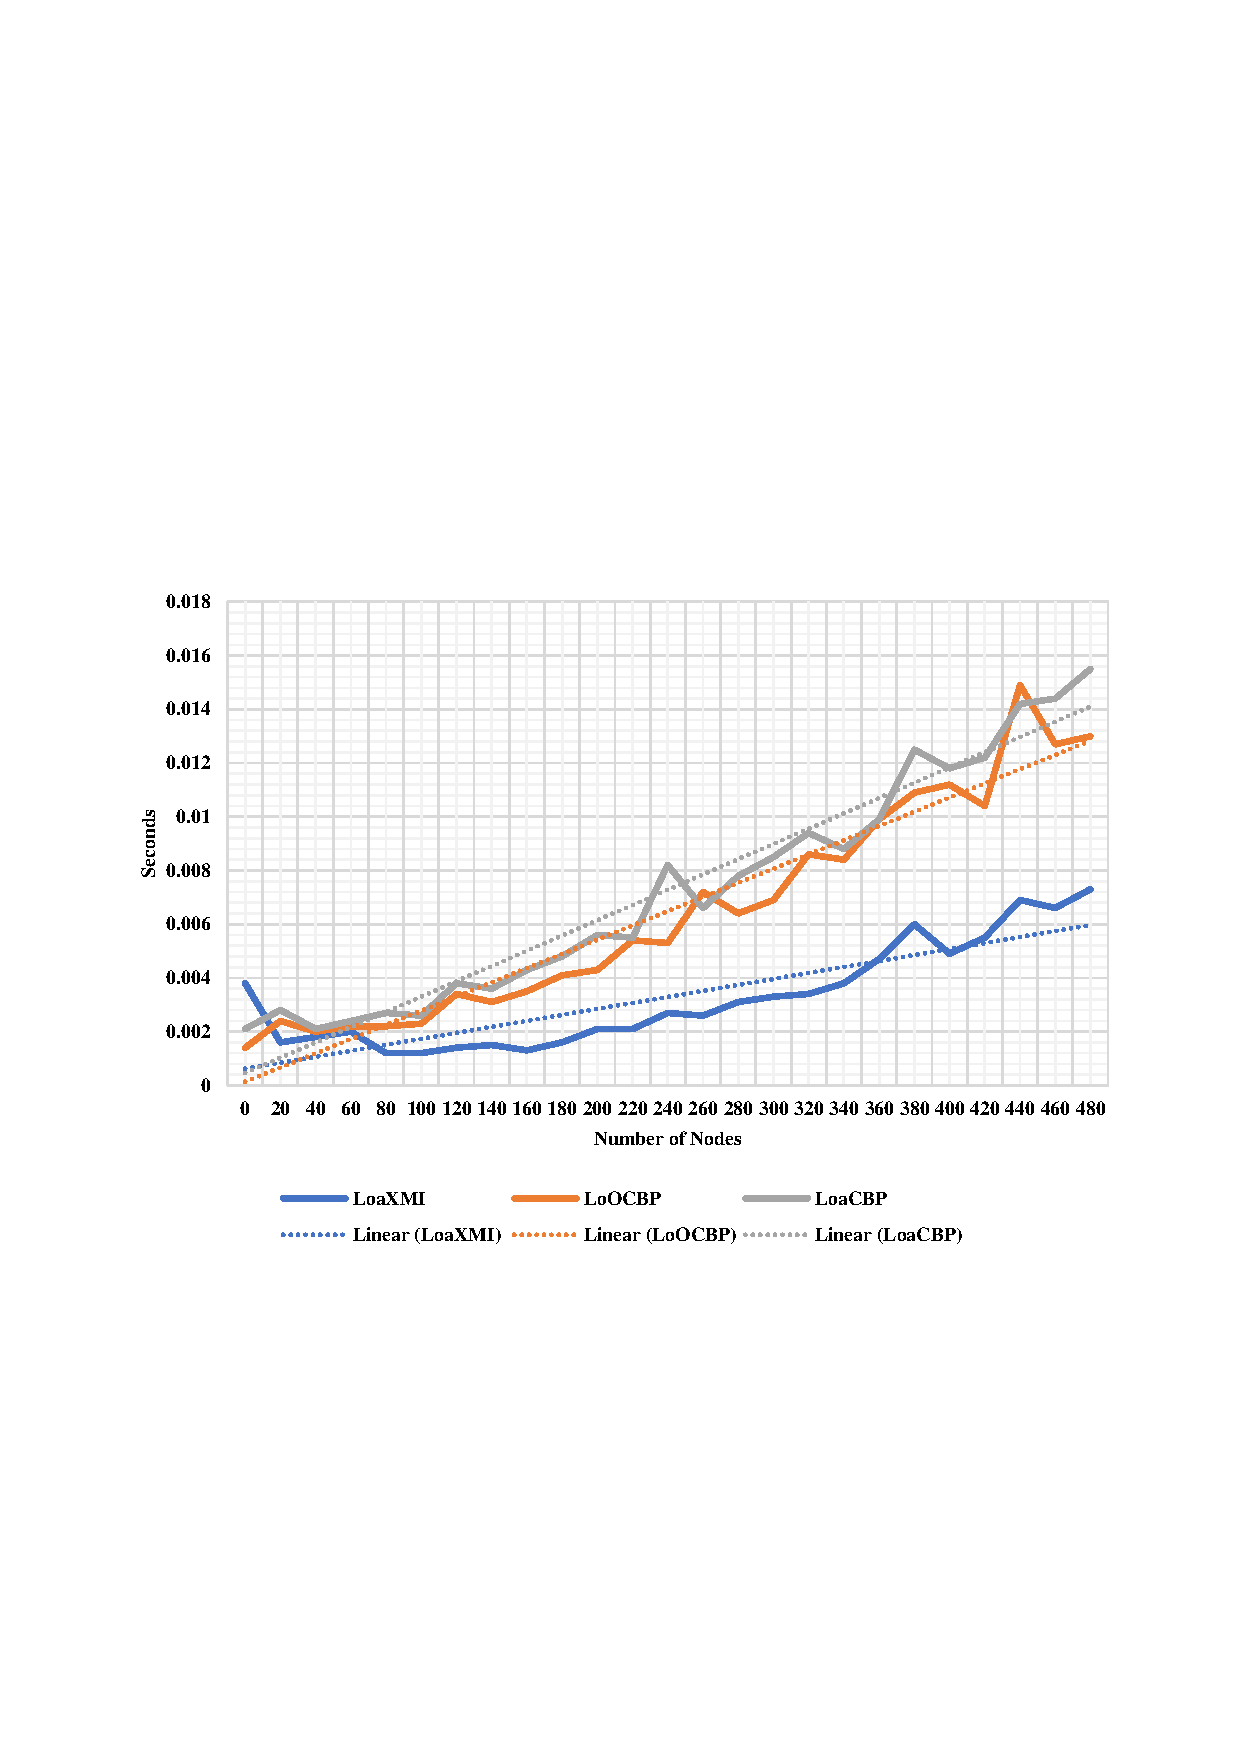
\includegraphics[width=\linewidth]{deep_tree}
\caption{Loading performance between loading XMI, optimised CBP, and CBP.}
\label{fig:deep_tree}
\end{figure}

\section{Related Work}

\section{Conclusions}


\cite{Lamport:LaTeX}.


\begin{acks}

\end{acks}


\bibliographystyle{ACM-Reference-Format}
\bibliography{ICSE-2018-bibliography} 

\end{document}
